\chapter{Preprocessing Patterns, Terms, and Top-Level Forms}



\section{Preprocessing Patterns: Introduction}
PyPltRedex mostly builds pattern trasformations and analyses on top of \texttt{PatternVisitor} class described in previous section and come in two varieties:

\begin{enumerate}
\item Ones that given a single pattern transform or analyze it.
\item Ones that given a \texttt{define-language} form perform transformation / analyses on all patterns in the form. This design decision allows for implementing passes not based on \texttt{PatternVisitor}
\end{enumerate}

TODO UML?



\section{Transformation: Pattern-Variable Resolution}
\label{section:pv-resolve}

\subsection{Algorithm}

Immediately after parsing the PLTRedex specification, it is unknown whether certain elements of a pattern are built-in patterns, non-terminal symbols or just literals. These elements are represented with \UnresolvedSymbol instances and will have to be resolved in one of the following ways: \BuiltInPatternNoArg, \NonTerminalNoArg, or \LiteralPatternNoArg.

If this transformation is being applied to \texttt{define-language} form, all sub-patterns that resolve to \LiteralPatternNoArg \space need to be stored in set $V$ (initially empty) which is the set of all variables used by the given language. After applying the transformation, \texttt{define-language} $l$ form has to be annotated with $V$ - \MakeAnnotation{$l$}{"ReservedVariables"}{$V$}.

Given \LetDefineLanguage{$l$}, let $\mathit{Nt_{l}}$ be the set of all non-terminal symbols of the language. Given string $\mathit{sym}$, the prefix of $\mathit{sym}$ needs to be extracted. Let $\mathit{prefix_{sym}}$ be a string of characters up to the first occurrence of an underscore character in $\mathit{sym}$. There are several cases to consider.

\begin{itemize}
\item $\mathit{prefix_{sym}}$ does not exist; there are no underscore characters in $\mathit{sym}$. Let $\mathit{prefix_{sym}=sym}$.
\item $\mathit{prefix_{sym}}$ is empty; the first character of $\mathit{sym}$ is underscore. Raise an Exception because PLTRedex doesn't consider such symbols valid.
\item Otherwise, $\mathit{prefix_{sym}}$ is the prefix.
\end{itemize}

The resolution algorithm proceeds in the following manner. The pattern is traversed recursively. When coming across \UnresolvedSymbol \space node, extract $\mathit{prefix_{sym}}$. One of the following cases may happen.

\begin{itemize}
\item Prefix is \texttt{number}, return \BuiltInPattern[Number][$\mathit{sym}$][false].
\item Prefix is \texttt{integer}, return \BuiltInPattern[Integer][$\mathit{sym}$][false].
\item Prefix is \texttt{real}, return \BuiltInPattern[Real][$\mathit{sym}$][false].
\item Prefix is \texttt{natural}, return \BuiltInPattern[Natural][$\mathit{sym}$][false].
\item Prefix is \texttt{string}, return \BuiltInPattern[String][$\mathit{sym}$][false].
\item Prefix is \texttt{boolean}, return \BuiltInPattern[Boolean][$\mathit{sym}$][false].
\item Prefix is \texttt{variable-not-otherwise-mentioned}, \\ return \BuiltInPattern[Variable][$\mathit{sym}$][false]
\item Prefix is \texttt{hole}. Since PLTRedex doesn't allow underscores for \texttt{hole} patterns check if $\mathit{prefix(sym) \neq sym}$ and raise an Exception accordingly. \\ Return \BuiltInPattern[Hole][$\mathit{sym}$][false].
\item $\mathit{prefix_{sym} \in Nt_l}$, return \NonTerminal[$\mathit{prefix_{sym}}$][$\mathit{sym}$][false].
\item Finally, ensure that symbol does not contain underscores. PLTRedex only allows underscores after non-terminal symbols and built-in patterns. Abort compilation process if that is the case. Otherwise, $V=V\cup\{\mathit{sym}\}$ and return \LiteralPattern[Variable][$\mathit{sym}$][false]
\end{itemize}

\subsection{Example}

\begin{figure}[ht]
	\makebox[\textwidth][c] { 
		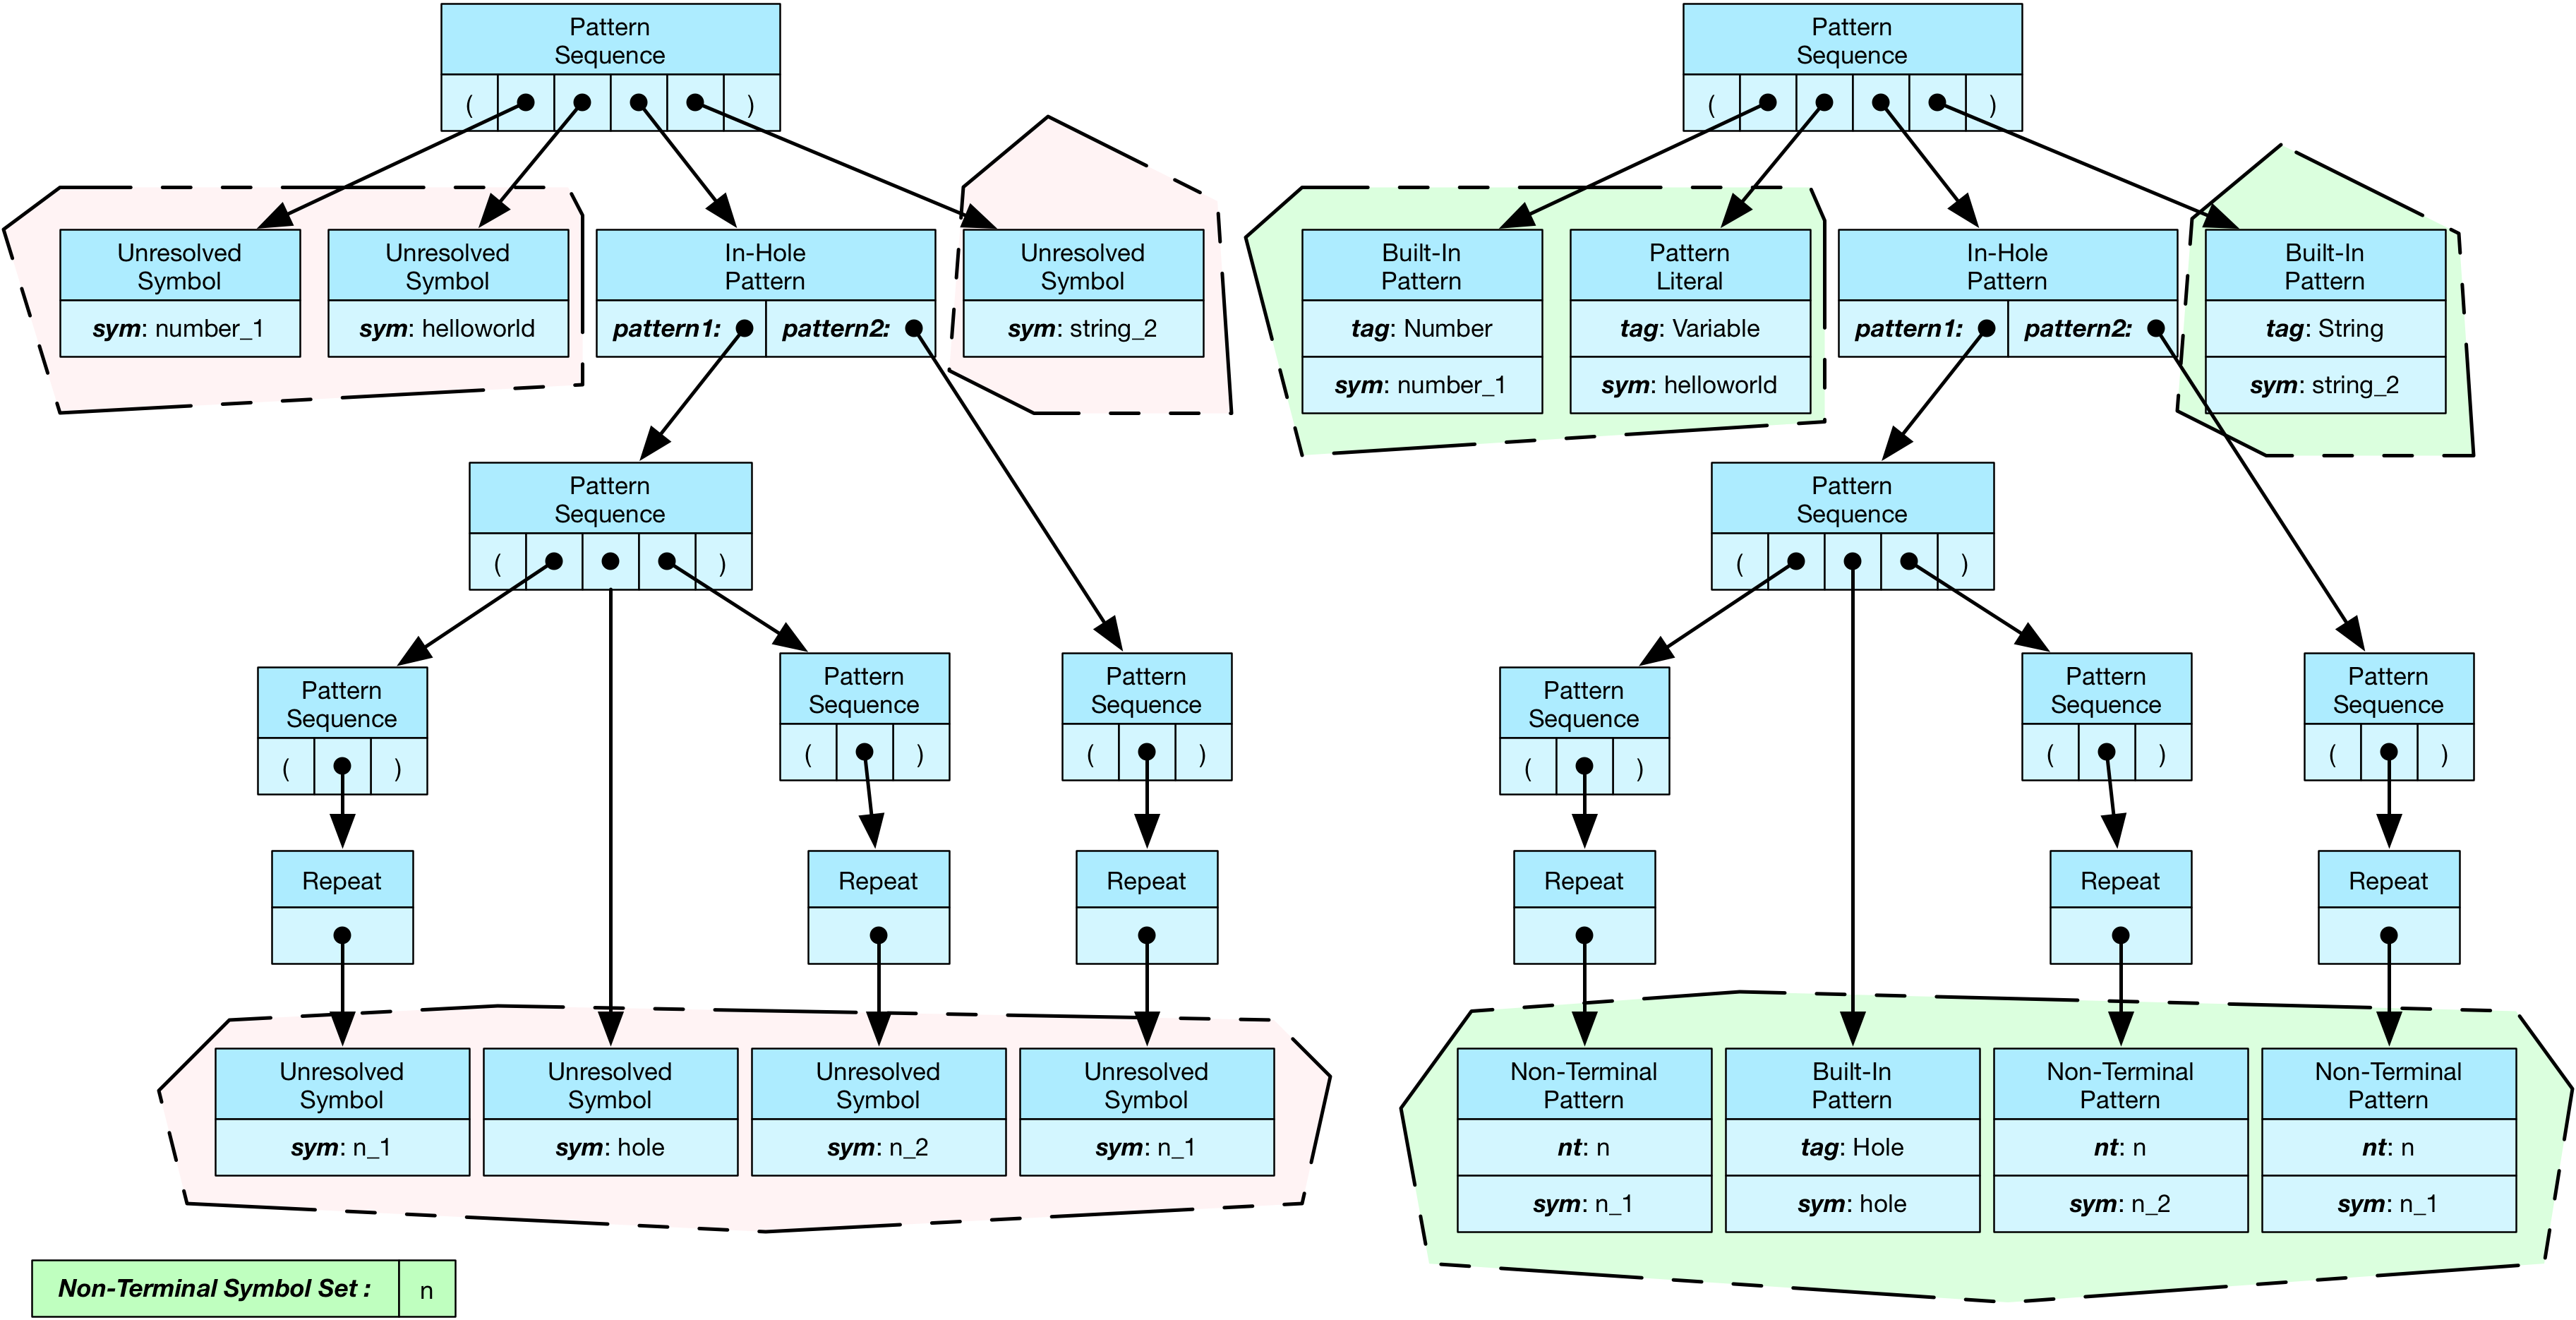
\includegraphics[scale=0.13]{transformation-pattern-resolvesym.png}
	}
\caption{Pattern before and after pattern variable resolution.}
\label{transformation-pattern-resolvesym}
\end{figure}

Figure \ref{transformation-pattern-resolvesym} shows an effect of transformation on pattern \texttt{(number\_1\ helloworld\ (in-hole\ ((n\_1\ ...)\ hole\ (n\_2\ ...))\ (n\_1\ ...))\ string\_2)}. Assume the related \texttt{define-language} has a single non-terminal \texttt{n}. Initially the pattern has six unresolved symbols - \texttt{number\_1}, \texttt{helloworld}, \texttt{n\_1}, \texttt{n\_2}, \texttt{hole} and \texttt{string\_2}. \texttt{number\_1}, \texttt{string\_2}, and \texttt{hole} become \texttt{BuiltInPattern} with appropriate tags,  \texttt{n\_1} and \texttt{n\_2} turn into non-terminals because prefix \texttt{n} is in the set of non-terminal symbols of given \texttt{define-language} and \texttt{helloworld} becomes a \texttt{LiteralPattern} with tag \texttt{Variable}. If this pattern were a part of \texttt{define-language}, \texttt{helloworld} would have been included into set $V$.

\section{Transformation: Identifier Rewriting}

\subsection{Motivation}

Recall that for patterns in \DefineLanguageNoArg constraint-checking is not performed. This means, for instance, that in this context patterns \texttt{(+ e e)} as \texttt{(+ e\_1 e\_1)} are equivalent. Due to design of \texttt{Match} class described in Section TODO, PyPltRedex needs to modify all such pattern-variables to be unique. Given pattern variable $pv$, $prefix_{pv}$ (defined in Section TODO) is extracted and concatenated with some previously unused integer - $freshint()$. 

\subsection{Algorithm}
Given \LetDefineLanguage{$l$}, each pattern in $NtDefinition$ is visited recursively.
\begin{itemize}
\item Given \BuiltInPattern, \\ return \BuiltInPattern[$tag$][$prefix_{pv}+freshint()$][false].
\item Given \NonTerminal, \\ return \NonTerminal[$nt$][$prefix_{pv}+freshint()$][false].
\end{itemize}

\subsection{Example}

Figure \ref{id-rewrite-example} shows an example of the transformation on \DefineLanguage form. To all non-terminals \texttt{e}, \texttt{n} and built-in pattern \texttt{number} numerical suffixes are added.

\begin{figure}[h]
	\begin{minipage}{0.5\linewidth}
		\centering
		\begin{minted}[tabsize=2,obeytabs,escapeinside=||,mathescape=true,fontsize=\small]{Racket}
(define-language L
	(e ::= (+ |\colorbox{identbefore}{e} \colorbox{identbefore}{e}|) 
	       (* |\colorbox{identbefore}{e} \colorbox{identbefore}{e}|) |\colorbox{identbefore}{n}|)
	(n ::= |\colorbox{identbefore}{number}|))
		\end{minted}
	\end{minipage}
	\begin{minipage}{0.5\linewidth}
		\centering
		\begin{minted}[tabsize=2,obeytabs,escapeinside=||,mathescape=true,fontsize=\small]{Racket}
(define-language L
	(e ::= (+ |\colorbox{identafter}{e\_0} \colorbox{identafter}{e\_1}|) 
	       (* |\colorbox{identafter}{e\_2} \colorbox{identafter}{e\_3}|) |\colorbox{identafter}{n\_0}|)
	(n ::= |\colorbox{identafter}{number\_0}|))
		\end{minted}
	\end{minipage}
	\caption{\texttt{define-language} before and afte renaming of identifiers.}
	\label{id-rewrite-example}
\end{figure}



\section{Ellipsis Depth Checking}

\subsection{Motivation}

Pattern-variables with the same symbol should be under a consistent number of ellipses. For example, in pattern \texttt{(((n\_1 ...) n\_1) ...)} the pattern variable \texttt{n\_1} is not under a consistent number of ellipses - one ellipses has \textit{ellipsis depth} of one, whereas the other is two. Such invalid patterns should be reported during the compilation process.

In addition, after pattern matching, the pattern-variables are plugged into term-templates and the ellipsis depth of each pattern-variable is needed to ensure that given term-template is well-formed.

\subsection{Pattern Traversal}

During pattern traversal, the following need to be maintained:

\begin{enumerate}
\item
Let $n$ be \textbf{number of ellipses} on the path from the root of the pattern to some child sub-pattern. $n$ is modified accordingly when visiting patterns of king \RepeatNoArg.

\item Association between pattern-variable $pv$ and its ellipsis depth $d$. Let $E=\emptyset$ containing pairs $(pv, d)$.
\end{enumerate}

Given some pattern $p$, \Visit{$p$}. The following kinds of $p$ are of interest.
\begin{itemize}
\item $p=$\PatternRepeat. Let $n=n+1$, \Visit{$p_r$}, and then let $n=n-1$.
\item $p$=\BuiltInPattern Check if there exists a pair $(pv, d) \in E$. If it does not, $E = E \cup \{ (pv, d) \}$. Otherwise, if $n \neq d$, then $pv$ has inconsistent ellipsis depth and an Exception is raised.
\item $p$=\NonTerminal is handled in the same way as \BuiltInPatternNoArg.
\end{itemize}

Finally, the pattern $p$ has to be annotated with $E$ - \MakeAnnotation{$p$}{"EllipsisDepths"}{$E$}.

\section{DefineLanguage: Non-Terminal Cycle Checking}

\subsection{Motivation}
PltRedex doesn't allow language definitions such as the one in Figure \ref{dl-ntcyclegraph}.

\begin{figure}[H]
\begin{minipage}{0.45\linewidth}
	\centering
\begin{minted}[tabsize=1,obeytabs,escapeinside=||,mathescape=true,linenos,fontsize=\small]{racket}
(define-language L
	(e ::= (e e) n)
	(n ::= (n n) number p)
	(p ::= (p p) real e))
	(s ::= string)
\end{minted}
\end{minipage}
\begin{minipage}{0.45\linewidth}
	\centering
	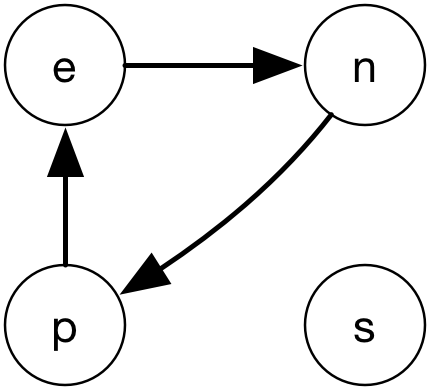
\includegraphics[scale=0.18]{transformation-pattern-ntgraph.png}
\end{minipage}
	\caption{\texttt{define-language} and its non-terminal graph}
	\label{dl-ntcyclegraph}
\end{figure}

The problem with the language above (aside from it being completely useless) is a cycle of non-terminals $n \rightarrow p \rightarrow e$. When testing if some term is a non-terminal, a term is matched against every pattern in a non-terminal definition. For example, given term \texttt{String("hello world")}, it is matched against non-terminal \texttt{e}. Since  the term doesn't match the pattern \texttt{(e e)}, non-terminal \texttt{n} is then matched. Since the term doesn't match any patterns here either, non-terminal \texttt{p} is then matched. Similarly, the term doesn't match any patterns here either, \texttt{e} is then matched, but that's where the matching has started and thus \textit{infinite recursion} becomes an issue. Languages need to be analyzed for presence of non-terminal cycles.

\subsection{Algorithm}
To detect such cycles, \DefineLanguageNoArg \space needs to be interpreted as a directed graph and some cycle-detecting algorithm must be used. The graph is constructed in the following manner.

\begin{enumerate}
\item
For each \NtDefinitionN[n], create a vertex labeled $n$.
\item
For $p_1, ..., p_n$, if $p_i$ is \NtDefinitionN[m], create the edge $n\rightarrow m$.
\end{enumerate}


To detect cycles, depth-first-search is employed. Vertices in the graph can be assigned one of three colors:

\begin{itemize}
\item

\textbf{White} - meaning the vertex hasn't been visited before. All vertices are initially assigned this color.

\item
\textbf{Gray} - meaning successors of the vertex $v$ are still being visited. When $v$ is visited for the first time, $color(v)$ becomes \textbf{Gray}.
\item
\textbf{Black} - meaning all successors of the vertex $v$ have been explored.
\end{itemize}



The detection of cycles is done through vertex coloring. For example, if during depth-first-traversal vertex $v$ is encountered with \DFSColor{$v$}{Gray}, this means that there's a \textbf{back-edge} in the tree created by depth-first traversal. That is, back-edge $u \rightarrow v$ connects vertex $u$ to its predecessor in the depth-first-search tree $v$. Once such cycle is found, the error is reported and the compilation aborts.

To report a path of non-terminals that make up the cycle, a path of non-terminals has to be maintained. The path can be represented as a stack. Given starting vertex $v$, depth-first-search proceeds as follows:

\begin{enumerate}
\item If \DFSColor{$v$}{Gray}, report cycle and abort compilation.
\item If \DFSColor{$v$}{White}, set color to \textbf{Gray} and add $v$ to the path.
\item Visit each successor vertex $v^{\prime}$ recursively.
\item Set color of $v$ to \textbf{Black} and remove it from the path.
\end{enumerate}

Since the resulting non-terminal graphs may be disjoint, we need to keep track of visited vertices during traversal. Let $V$ be a set of vertices whose \DFSColor{$v$}{Black}. Thus, every time vertex $v$ changes its color to \textbf{Black}, $V = V \cup \{v\} $. Let $U$ be a set of vertices whose \DFSColor{$v$}{White}; that is, it initially contains all the non-terminals. The algorithm proceeds as follows:

\begin{enumerate}
\item
Pick a random vertex $u$ from set $U$. Create empty set $V$. Starting from $u$, perform depth-first-search as described above. Compute set difference - $U = U-V$.
\item
Continue until $U$ is empty.
\end{enumerate}

It should be noted that the algorithm described does not report all the cycles in the graph but the first one it manages to find. One improvement could be finding all cycles in the graph.

\subsection{Example}

Figure \ref{nt-cycle-example} demonstrates cycle searching using the graph shown in Figure \ref{dl-ntcyclegraph} starting from the non-terminal $s$. Initially $U=\{s,p,n,e\}$. Its color becomes \texttt{Gray} as seen in (a). Since it has no successor vertices, its color becomes \texttt{Black}, as seen in (b).

Since $V = \{ s \}$, $U=\{p,n,e\}$. Pick vertex $p$ for expansion and color it \texttt{Gray}. Then, visit the only successor of $s$, vertex $e$ and color it \texttt{Gray}. Visit the only successor of $e$, vertex $n$ and color it \texttt{Gray}. Finally, visit the only successor of $n$, vertex $p$. But since it is already colored \texttt{Gray}, the cycle  $p \rightarrow e \rightarrow n$ has been found and a compilation error should be raised.

\begin{figure}[h]
\begin{subfigure}{0.32\linewidth}
	\centering
	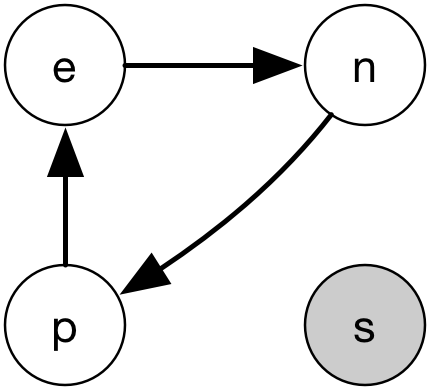
\includegraphics[scale=0.18]{transformation-pattern-ntgraph-example-1.png}
\end{subfigure}
\begin{subfigure}{0.32\linewidth}
	\centering
	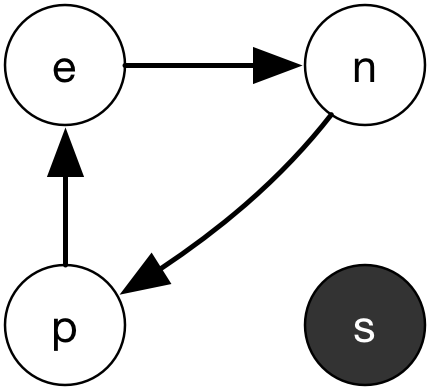
\includegraphics[scale=0.18]{transformation-pattern-ntgraph-example-2.png}
\end{subfigure}
\begin{subfigure}{0.32\linewidth}
	\centering
	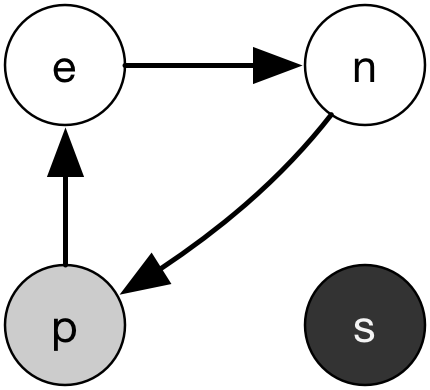
\includegraphics[scale=0.18]{transformation-pattern-ntgraph-example-3.png}
\end{subfigure}
\newline
\begin{subfigure}{0.32\linewidth}
	\centering
	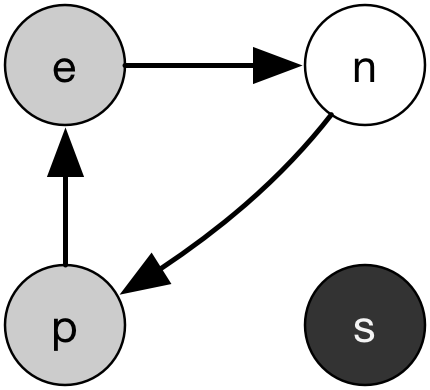
\includegraphics[scale=0.18]{transformation-pattern-ntgraph-example-4.png}
\end{subfigure}
\begin{subfigure}{0.32\linewidth}
	\centering
	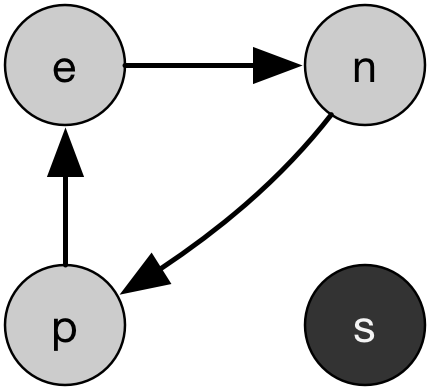
\includegraphics[scale=0.18]{transformation-pattern-ntgraph-example-5.png}
\end{subfigure}
\begin{subfigure}{0.32\linewidth}
	\centering
	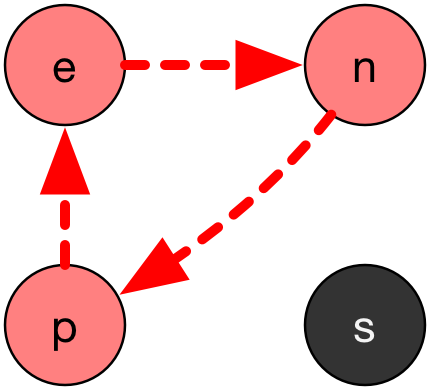
\includegraphics[scale=0.18]{transformation-pattern-ntgraph-example-6.png}
\end{subfigure}
\caption{Cycle searching using DFS.}
\label{nt-cycle-example}
\end{figure}

\section{Hole Reachability}

The pattern \InHolePattern requires $p_1$ to match exactly one \lstinline{hole} term. The main problem is counting a number of holes matched by non-terminal symbols of the language. Consider the language \lstinline{MatchesManyHoles} listed below.

\begin{lstlisting}
(define-language MatchesManyHoles
	(n ::= number)
	(P ::= E (n ... E ...))
	(E ::= (+ E P) (+ n E) hole))
\end{lstlisting}

To compute value for  the non-terminal \lstinline{E}, an analysis of pattern \lstinline{(+ E P)} is required but the value of \lstinline{E} is not yet known. Moreover, computing a single value that represents number of holes is insufficient; pattern lstinline{(E ...)} may match zero or many holes. Thus, a \textbf{minimum} and \textbf{maximum} number of holes matched by some pattern must be computed.

\subsection{Graph Modeling}

Graph consists of two parts - \textbf{outer-nodes} and \textbf{inner-nodes}.

Outer-nodes are a stand-in for the pattern and come in four different varieties:

\begin{itemize}
\item \lstinline{Sequence} representing pattern-sequences.
\item \lstinline{Repeat} representing ellipses.
\item \lstinline{LeafHole} representing the pattern \lstinline{hole}.
\item \lstinline{LeafNotHole} representing any other pattern except \InHolePattern
\end{itemize}

Inner-nodes are stored in \lstinline{Sequence} and \lstinline{Repeat} outer-nodes and act as non-terminal references. Each inner-node has a set of outer-node successors pointing to a set of expressions that the non-terminal matches.

Graph for language defined above can be seen in the following figure:
TODO

\subsection{Graph Construction}

Constructing the graph involves two stages:
\begin{enumerate}
\item
Creation of outer nodes for each top-level pattern such as `(+ E P)` or `hole`.
\item
Creation of inner nodes and edges from inner to outer nodes. If the outer node is a `Sequence` and it contains other sequences or ellipses, additional creation of outer-nodes will be required.
\end{enumerate}


\subsection{Creation of Outer Nodes}

A mapping of `M` has to be maintained between patterns in non-terminal definition. For each non-terminal definition `N` let `E\_N = \{\}` be a set storing top-level non-terminal references. For example, in the language described above for non-terminal definition `P` the only such reference is `E`.

Each non-terminal definition `N` is visited and we may come across the following patterns.
\begin{itemize}

\item
\BuiltInPattern. If kind is `Hole` then `n = LeafHole` node is created.  Otherwise, `n = LeafNotHole` node is created. Thus, `M = M union {(p, n)}`.
\item
\Nt. This means that `N` is also `nt` and thus all expressions in non-terminal definition of `nt` should also be reachable from any inner-node that reaches expressions in `N`. Thus, `E\_N = E\_N union {nt}`.
\item
\InHolePattern. Raise compilation error and quit. This, however, is not actual behavior of the PltRedex. (TODO explain why we handle it differently?)
* `p = PatternSequence(pattern ...)`. If length of `p` is zero, then `n = LeafNotHole`, otherwise `n = Sequence`. Thus, `M = M union {(p, n)}`.
\end{itemize}

Note that creating multiple `LeafHole` or `LeafNotHole` nodes is not necessary and existing nodes of these kinds can be reused. This means that the graph may have at most two leaf nodes.


\subsection{Creation of Inner Nodes and Edges}

The only top-level pattern kind that may contain inner nodes at this point is `Sequence` and thus they need to be visited. One thing that needs to be maintained is the stack `S` of outer-nodes where inner-nodes are to be stored.

For each non-terminal definition `N` and each pattern $p_i$, if $p_i$ is `PatSequence`, retrieve `M[$p_i$]` from the mapping and place on top of the stack S. For each subpattern $q_i$ in $p_i$, visit $q_i$.

\begin{itemize}
\item
\PatternSequence. Create outer-node `Sequence` `s` for `p`; create inner node `i`; add edge `i->s`. Retrieve parent outer-node `O` and add node `i` to it. Append `s` to the stack `S`. For each child pattern $c_i$ of `p`, recursively visit each $c_i$. Pop topmost element off the stack `S`.

\item
* \Repeat. Create outer-node `Repeat` `r` for `p`, create inner node `i`, add edge `i->r`. Retrieve parent outer-node `O` and add node `i` to it. Append `r` to the stack `S`. Visit child pattern `c` of `p`. Pop topmost element off the stack `S`.

\item
\InHolePattern Raise compilation error and quit.

\item
\BuiltInPattern. Create inner node `i`. If kind is Hole then let s = LeafHole, otherwise s = LeafNotHole. Create edge `i->s`.  Retreieve parent outer-node `O` from the top of the stack and add node `i` to it.

\item
\Nt Create inner node `i`. For each pattern in non-terminal definition of `nt`, retrieve outer-node `o` from the mapping `M` and create edge `i->o`. Do the same for each non-terminal in the set `E\_nt`. Retrieve outer-node `O` from the stack and append `i` to it.

\end{itemize}

\subsection{Minimal/Maximal Value Representation and Arithmetic}

Minimum / maximum number of holes can be one of the following: `Zero`, `One`, `Many` (i.e. >= 2) and `Uninitialized` indicating said value should not be used for computation just yet.

Furthermore, three operators need to be defined - `+`, `min`, `max`. Assume Zero = 0, One = 1, Many = 2 and Uninitialized = 3

Addition operation.

\begin{align}
	a + b =
	\begin{cases}
		3 \text{ if } a = 3 \text{ and } b = 3 \\
		a \text{ if } b = 3 \\
		b \text{ if } a = 3 \\
		min(a + b, 2)
	\end{cases}
\end{align}

Min operation:

\begin{align}
	min(a,b) =
	\begin{cases}
		3 \text{ if } a = 3 \text{ and } b = 3 \\
		a \text{ if } b = 3 \\
		b \text{ if } a = 3 \\
		min(a, b)
	\end{cases}
\end{align}

Max operation:
\begin{align}
	max(a, b) =
	\begin{cases}
		3 \text{ if } a = 3 \text{ and } b = 3 \\
		a \text{ if } b = 3 \\
		b \text{ if } a = 3 \\
		max(a, b)
	\end{cases}
\end{align}


\subsection{Computation of Values}
Min/max values are computed both for inner-nodes and outer-nodes. First, they have to be initialized.

\begin{itemize}
\item
Inner nodes are initialized with (Uninitialized, Uninitialized)
\item
`Sequence` and `Repeat` outer nodes are initialized with (Uninitialized, Uninitialized)
\item
`LeafHole` outer node is initialized with (One, One)
\item
`LeafNotHole` outer node is initialized with (One, One)
\end{itemize}


Given initial values $min_inner$, $max_inner$ of some inner-node  and new values $v_1$, $v_2$, $min_inner = min(min_inner, v1)$, $max_inner = max(max_inner, v2)$.


Given outer-node `o`, there are a few cases to consider.

\begin{itemize}
\item
`LeafHole` and `LeafNotHole` - its min/max values are never updated.
\item
* `Sequence` - $min_o = \sum_{i in inner(o)} min_i$ and $max_o = \sum_{i in inner(o)} max_i$. Summation is described above.
\item
* `Repeat` - $min_o = Zero$, $max_o = Many if max_inner = One or max_inner = Many else Zero$.
\end{itemize}

\subsection{Hole Reachability Algorithm}

Before initiating graph traversal, verify if `LeafHole` node is actually in `V`. If there is no such node, that means the source pattern does not match any `hole` and thus each non-terminal should be annotated with `Zero,Zero` number of holes.

Otherwise, the graph is traversed in reverse direction starting from nodes `LeafHole` and `LeafNotHole` using breadth-first strategy. Maintain queue Q that initially stores all `LeafHole` and `LeafNotHole` nodes.

The algorithm is as follows:
\begin{enumerate}
\item
Remove outer node `o` from the queue `Q`.
\item
* For each inner-node `i` such that `i->o`:
	\begin{enumerate}
	\item
	if `parent(i) = o` then $update(i, o_min, o_max)$ and `update(o)`. This means that if the inner node contains an edge to the outer-node `o` `i` is a child of, thus can be considered a "self-loop". The reason for doing this will be discussed later. (TODO is this actually needed aside from really degenerate patterns?)
	\end{enumerate}

\item
For each inner-node `i` such that `i->o`:
	\begin{enumerate}
	\item
	if `parent(i) != o`, $update(i, o_min, o_max)$ and update(o). If values of $o_min, o_max$ are different from ones before update operation, add `o` to the queue `Q`.
	\end{enumerate}

\item
* Repeat until queue `Q` is empty.

\end{enumerate}


\subsection{Computing Min/max values for non-terminal definition}

Given non-terminal definition `nt` and set of patterns `P` it matches, $min_nt = max_nt = Uninitialized$. Then, $min_nt = \min_{i in P} min_i$ and $max_nt = \max_{i in P} max_i$.Note that some parrern `i` in `P` may be Nt, in which case $min_i$ and $max_i$ for non-terminal definition `i` first. By ensuring that language contains no non-terminal cycles, such recursive procedure s guaranteed to terminate.

After completing all computations, each non-terminal definition `nt` is annotated with corresponding $min_nt, max_nt$.


\subsection{Edge cases}.

This algorithm doesn't do one very specific thing - infinite terms and presence of `hole`. Consider the language below

\begin{lstlisting}
(define-lagnuge Infinite
     (P ::= (E))
     (E ::= P hole))
\end{lstlisting}

\subsection{Example}
TODO

\section{Pattern: \lstinline{in-hole} Pattern Checker}

Having computed `min/max` numbers for each non-terminal in the language, now the question of whether `pattern1` in pattern \InHolePattern actually matches exactly one hole. Doing so involves two stages: 

\begin{enumerate}
\item
Locating \InHolePattern in the top-level pattern.
\item
Checking if $p_1$ matches exactly one hole. Since $pattern1$ doesn't necessarily have to be a non-terminal, extra work will have to be required.
\end{enumerate}

\subsection{Checking pattern for number of holes}

Assuming \InHolePattern pattern has already found, $p_1$ has to be visited recursively. One of the following nodes may be visited.

\begin{itemize}
\item
\BuiltInPattern - if $t=$hole then $min_p = One, max_p = One$, otherwise $min_p = Zero, max_p=Zero$.

\item
\Nt. Read appropriate annotation from non-terminal definition in `define-language` and return values.

\item

\LiteralPattern min\_p = Zero, max\_p = Zero.

\item
\InHolePattern. Return $min_p = Zero, max_p = Zero$, this seems to be default PltRedex behaviour.

\item
\Repeat. Recursively visit the $p$ obtaining $min_p2$, $max_p2$. The logic for Repeat is identical to the one used in **Hole Reachability**; that is:
	\begin{itemize}
	\item
	$min_n = Zero$
	\item
	$max_p = Many if max_p2 = One or max_p2 = Many$
	\item
	$max_p = Zero$ otherwise
	\end{itemize}

\item
* \PatternSequence. Initially, $min_p$, $max_p = Unitialized$. Then, $min_p = \sum_{p_i in p} minp_i$. To obtain $minp_i$, $p_i$ has to be recursively visited.
\end{itemize}

\subsection{Example}
TODO

\section{Constraint Check Insertion}
As mentioned before, Redex supports a few different forms of constraint checking; however, for the initial PyRedex implementation only "equality of terms" constraint check will be supported. For example, in pattern `(number\_1 number\_1)` both bound terms must be the same, that is term `(1 1)` matches the pattern but `(1 2)` does not. 

However, the `Match` object does not store multiple bindings for the same symbol and thus assignable symbols seen in the pattern have to be renamed. In the example above, the pattern could become `(number\_1 number\_1\#1)`. Now both bound terms can be stored in the `Match` object.

Now, actual equality checks have to be inserted. Two obvious strategies could be employed here:

\begin{itemize}
\item
Perform constraint checking after the pattern has been matched entirely. For example, `(n\_1 n\_1\#1 n\_2 (Check n\_1 == n\_1\#1))`. The disadvantage of this strategy is that if pattern is large and something goes wrong in the beginning the rest of the pattern is still matched and lots of useless work is done. 

\item
Perform constraint checking the earliest time possible. This implies that by that time both terms have to be matched. Pattern `(n\_1 n\_1\#1 (Check n\_1 == n\_1\#1) n\_2)` is the example of such strategy. The disadvantage of this strategy is that assignable symbols under ellipsis will be checked multiple times. `(((number\_1 ...) (number\_1\#1 ...) (check number\_1 == number\_1\#1)) ...)`
\end{itemize}
The algorithm to be detailed below employs the second strategy.

Finally, since `Match` object now contains extra symbols such as `number\_1\#1` these will have to be removed after successfully matching the pattern.

\subsection{Algorithm}
To be able to insert constraint-checks all symbols to end up in `Match` object have to be known. Since certain symbols will be renamed, need to maintain a mapping between old symbol and new symbol. Additionally, maintain a set to store symbols that will have to be removed. The pattern is traversed recursively. 


\begin{itemize}
\item
\BuiltInPattern and \Nt. Generate a fresh symbol given template string `symbol\_\#`. If generated symbol is `symbol\_\#0` then original symbol is seen for the first time and thus remains unchanged. Otherwise, modify `BuildInPattern` and `Nt` by changing its symbol to a new one. Add new symbol to the set of the symbols to be removed. After processing the pattern, return a mapping `{tag : symbol}` if pattern is `BuildInPattern` or `{nt: symbol}` if pattern is `Nt`.

\item
\LiteralPattern contains to no assignable symbols and thus empty list is returned.

\item
\Repeat. Recursively visit $p$ and return its mapping. 

\item
\PatternSequence. If sequence contains no child patterns, return empty mapping. Otherwise, let `syms` be a mapping returned after visiting the first pattern. For each remaining pattern in the sequence:
	\begin{enumerate}
	\item
	Let `syms2` be a mapping returned after visiting the pattern.
	\item
	Let `syms` be a result of merging `syms` and `syms2` mappings; merging will be discussed below.
	\item
	Let `syms2merge` be a set containing pairs of symbols that have to be checked for equality obtained fter merging `syms` and `syms2` mappings. For each pair of symbols in `syms2merge` add `ConstraintCheck` node to the sequence, exactly after the current pattern. 
	\end{enumerate}

\item
\InHolePattern. Let `syms1`, `syms2` be mappings returned after visiting `pattern1` and `pattern2`, respectively. Let `syms` be a result of merging `syms` and `syms2` mappings, and let `syms2merge` be a set containing pairs of symbols. For each pair of symbols `(s1, s2)` in the set, create `cc\_i` = `ConstraintCheck(s1, s2)` node. Replace InHole pattern with `InHole(pattern1, pattern2, {cc\_0 ... cc\_i ... })`.
\end{itemize}

\subsection{Variable Merging}

Consider pattern `(number\_1 number\_1\#1 number\_1\#2)` and observe that after inserting constraint checks in the following way: `(number\_1 number\_1\#1 (number\_1 == number\_1\#1 ?) number\_1\#2 (number\_1 == number\_1\#2 ?) (number1\#1 == number\_1\#2 ?))` one of the comparisons it the end is superfluous since it's known that `(number\_1 == number\_1\#1)`. Thus, while merging mappings, only one assignable symbol has to be in resulting mapping.

Given two mappings $m1 = {k_i: sym1, k_j: sym2, ...}$ and $m2 = {q_i: sym, q_j: sym}$, compute ${k_0 ... k_i ... k_n}$ intersection ${q_0 ... q_i ... q_n}$. If some $p_i$ is in intersection, retrieve $m1[p_i]$ and $m2[p_i]$ and create pair out of retrieved elements. These symbols will require constraint checking. 

The resulting mapping is constructed in the following way:
\begin{itemize}
\item
If $p_i$ is in intersection, add ${p_i: m2[p_i]}$ to the mapping.
\item
For any $k_i$ that is not in intersection add ${k_i: m1[k_i]}$ to the mapping.
\item
For any $q_i$ that is not in intersection add ${q_i: m2[q_i]}$ to the mapping.
\end{itemize}

\subsection{Example}
TODO


\section{Pattern: Pattern-Variable Extraction}
\label{section:pv-extraction}

\subsection{Motivation}
Since \texttt{Match} instances are initialized with pattern-variables, all pattern-variables used by some pattern $p$ need to be known. 

\subsection{Term Traversal}
The algorithm recursively traverses the pattern and at each step returns a set of pattern-variables $V$. Given some pattern $p$, $V=$\Visit{$p$}. The following kinds of $p$ are of interest.

\begin{itemize}
\item $p=$\NonTerminal. Return $V = \{ pv \}$.
\item $p$=\BuiltInPattern. Return $V=\{ pv \}$.
\item $p$=\LiteralPattern. Return $V=\emptyset$.
\item $p$ = \PatternSequence. Return $V=\bigcup_{i=1}^{n}$\Visit{$p_i$}.
\item $p$ = \PatternRepeat. Let $V_r=$\Visit{$p_r$}. Need to annotate $p$ with $V_r$: \MakeAnnotation{$p$}{"PatternVariables"}{$V_r$}.
\item $p$ = \PatternInHole. Let $V_1=$\Visit{$p_1$} and  $V_2=$\Visit{$p_2$}. Annotate $p_1$ and $p_2$ with corresponding pattern-variable sets: \MakeAnnotation{$p_1$}{"PatternVariables"}{$V_1$} and \\ \MakeAnnotation{$p_2$}{"PatternVariables"}{$V_2$}. Return $V = V_1 \cup V_2$.
\end{itemize}

Finally, \MakeAnnotation{$p$}{"PatternVariables"}{$V$}.

\section{Term Template: Ellipsis Depth Checking}

As mentioned before, our goal is to resolve all ellipses at compile time by ensuring that there are no patterns under ellipses that do not have at least a single pattern variable. In addition, unresolved symbols must be resolved based on variables assigned in `Match` object. 

\subsection{Annotation}
At this stage, since pattern variables will need to be replaced with terms, inputs to term-templates are detected. This is done by annotating term-templates. The following annotations are introduced:

\begin{itemize}
\item
InArg(parameter\_name) - some pattern variable term-template or any of its child term-templates is replaced with term (or subterm) assigned to `parameter\_name`. 
\item
* `ReadMatch(parameter\_name, sym)` takes a term from `Match[sym]` and assigns in to `parameter\_name`. If there happens to be some child term-template containing pattern variable with value `sym`, this means that all term-templates on the path to that specific child term-template will be annotated with `InArg(parameter-name)`.
\item
* `ForEach(parameter\_name)` annotation is added to \TermRepeat term-templates and means that every element of the term sequence assigned to `parameter\_name` must be plugged in child term-template assuming the term has compatible ellipsis depth.
\end{itemize}

Explanation of `parameter\_name` is needed. These are used to prevent name collisions ... (TODO exammple)

\subsection{Algorithm}

To perform annotation, a path of term-templates must be maintained to be able to count all ellipsis on the path to the root term-template. A structure of `Match` object (i.e. a list of variables and ellipsis depth of matched terms) is also known (from chapter???). Given all, start recursive term-traversal.

When any term-template is visited, it is added to the top of the path stack. When term-template and its child term-templates have been visited, top-most element is popped from the stack. Now we consider term-templates that may be visited.
\begin{itemize}

\item
\TermUnresolvedSymbol. First, check if symbol is present in `Match` object. If it isn't then the symbol cannot be `PatternVariable` but `TermLiteral.Variable`. Otherwise, it is a pattern variable and thus number of ellipsis on the path must be greater or equal to the expected ellipsis depth. There are multiple cases to consider.
	\begin{itemize}
	\item
	Expected ellipsis depth is zero. Let `n` be a fresh symbol containing pattern variable symbol (e.g. if symbol is `e` then freshsymbol could be `e1`)  `PatternVariable` is then annotated with `MatchRead(n, sym)` and returned.
	\item
	Expected ellipsis depth is greater that zero. Annotate pattern variable with `InArg(n)`. Initialize actual ellipsis depth to zero. We need to inspect the contents of the path to be able to determine actual ellipsis depth of the pattern variable. Top-most element of the path stack is `UnresolvedSymbol` and is ignored. Iterate over the path in reverse order. 
		\begin{enumerate}
		\item
		If current element is `TermSequence` or `InHole` and actual depth not equal expected depth add `InArg(n)` annotation.
		\item
		If current element is `TermSequence` or `InHole` and actual depth is equal to expected depth add `ReadMatch(n, sym)` annotation and return `PatternVariable`.
		\item
		If current element is `Repeat` then add `ForEach(n)` annotation and increment actual ellipsis depth.
		\end{enumerate}

	  Othewise, we have iterated through the entire path and failed to consume expected number of ellipses. Raise exception. Note that path does not contain `PythonCall`. Reasons for this will be explained later.
	\end{itemize}
\item
\TermRepeat First, recursively visit child term-template. Check if `Repeat` is annotated with `ForEach`. If it is not, then it means there are no pattern variables in child term-template and thus `Repeat` is not well-formed. Raise exception.
\item
\TermSequence Recursively visit each child template and return `TermSequence`. There is nothing left to do here.
\item
\TermInHole Recurisvely visit both child patterns and return `InHole`.
\item
\PythonCall Recall that `PythonCall` accepts a sequence of term-templates and calls Python function with resulting terms as arguments. These child term-templates must be visited recursively but path must be emptied out and then restored after visiting child term-template. The reason for that is because term-templates such as `(,(add (term n\_1) (term n\_2)) ...), with terms bound to `n\_1` and `n\_2` both having ellipsis depth of two, are invalid. This is also the reason why `PythonCall` is never encountered while iterating over the path while processing `UnresolvedSymbol`.
\end{itemize}


\subsection{Example}
TODO



\section{Term-Template: Rewriting Metafunction Applications}

Since metafunction applications have the following shape - \texttt{(metafunction-name\ term-template\ ...)} these can be detected quite trivially given a list of defined metafunctions. 

\subsection{Algorithm}
Let $Mf$ be the set of metafunction names. Let $t$ be some term-template, \Visit{$t$}. 
\begin{itemize}
\item $t=$\space \TermSequence. Check if $t_1$ is \TermLiteral\space with $kind=$\space Variable and $v \in Mf$. Return \\ \ApplyMetafunction[$v$][$t$][false] if that is the case, handling annotations as described below; otherwise return $t$. 

$t$ may contain \texttt{InArg} and \texttt{MatchRead} annotations and they are modified in the following way:
\begin{itemize}
\item
\texttt{InArg} annotations are left intact. Signatures of both \texttt{TermSequence} and \texttt{ApplyMetafunctions} must match.
\item
\texttt{MatchRead} annotations can be safely removed. None of such variable assignments are used to generate $t$.
\end{itemize}
\end{itemize}
\subsection{Example}
The example shown in Figure \ref{transformation-term-mfapply} displays the transformation described above given a set of meta-function names only containing a single \texttt{set-contains?}. Since the first element of \texttt{TermSequence} is a \texttt{Variable} term-template with suitable name, an additional \texttt{MetafunctionApplication} term is added.

\begin{figure}[H]
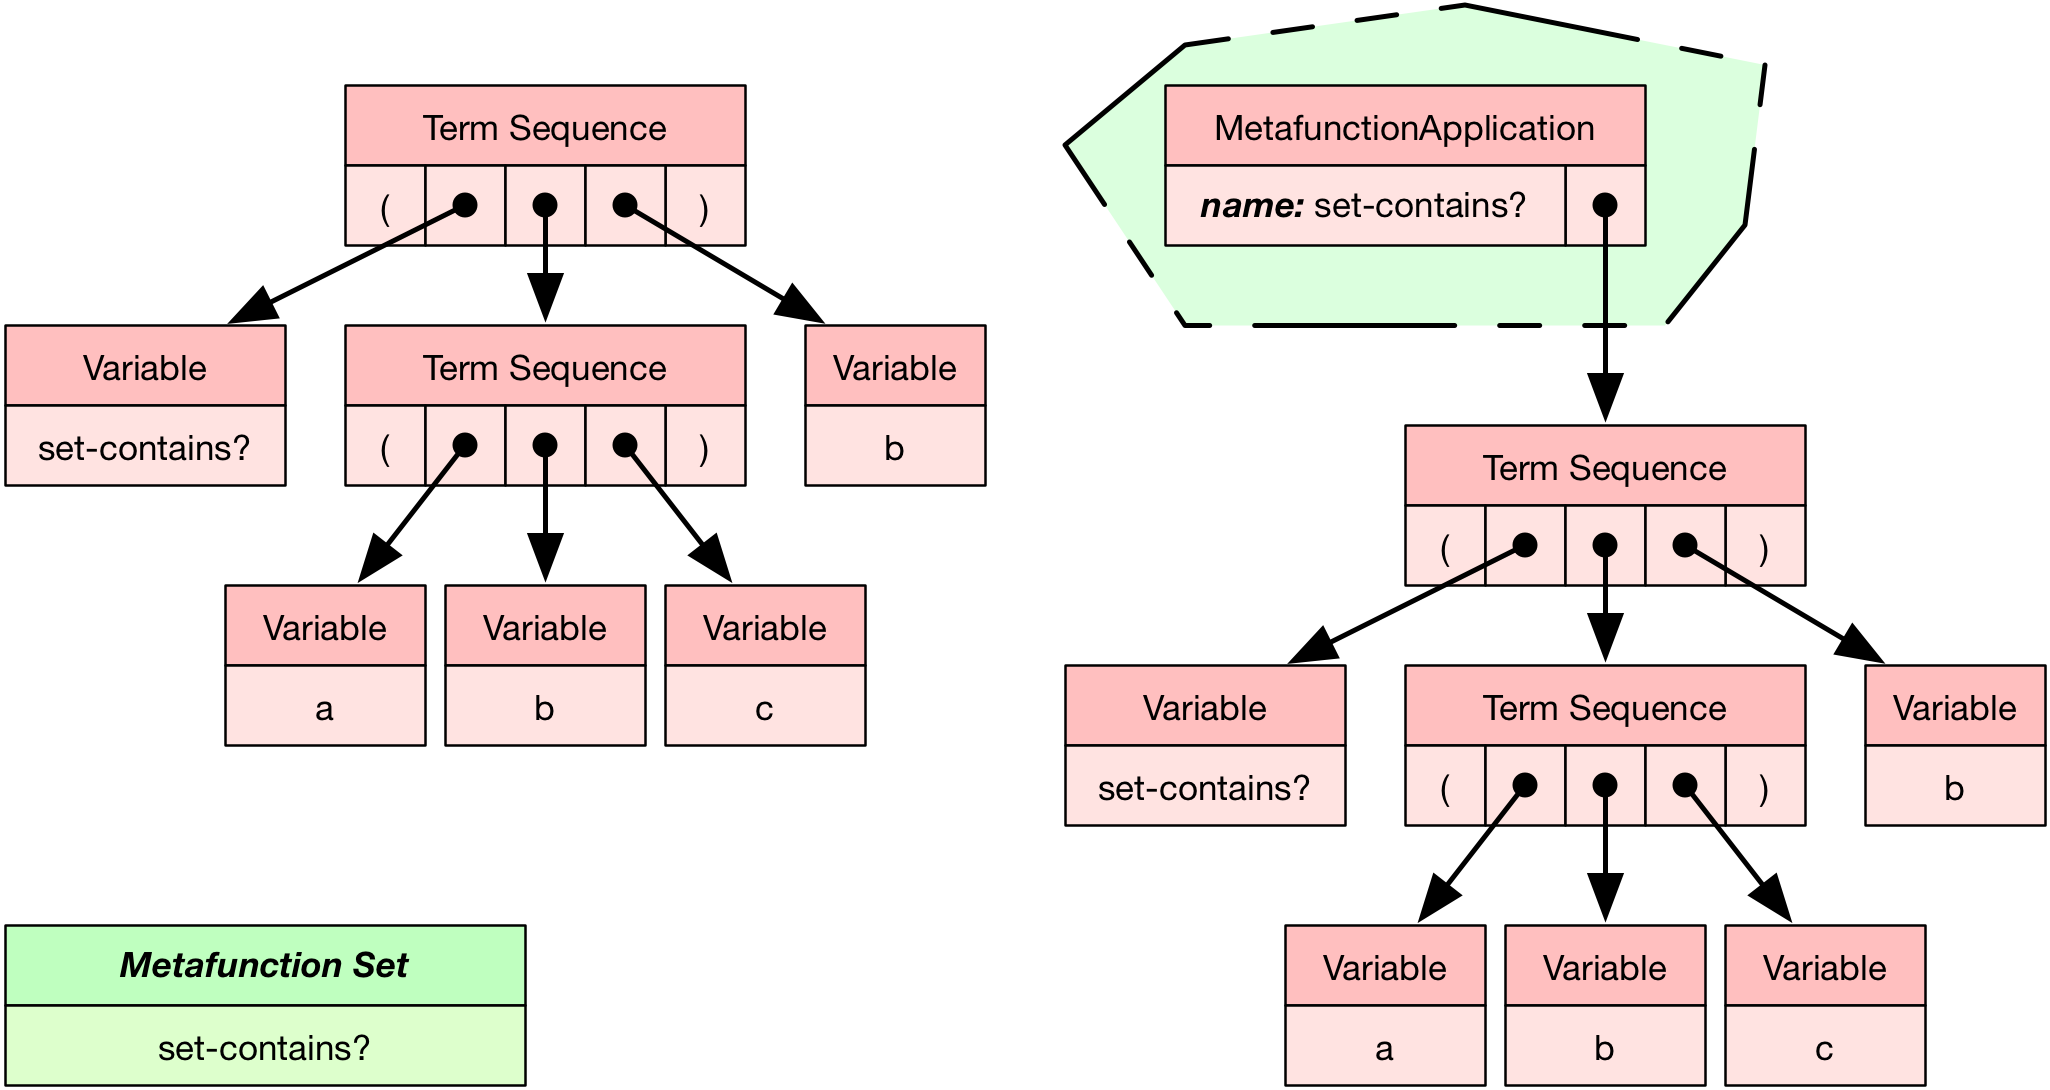
\includegraphics[scale=0.20]{transformation-term-mfapply.png}
\caption{Term-template before and after applying metafunctions.}
\label{transformation-term-mfapply}
\end{figure}

\section{Preprocessing Top-Level Forms}

Having defined and explained transformation/analysis passes for both patterns and term-templates, these are combined according to the needs of top-level forms.

Identify three strategies for processing patterns.

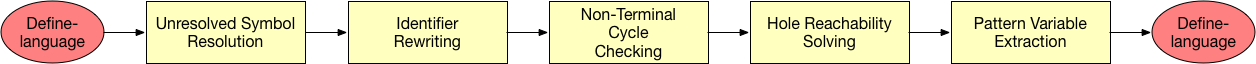
\includegraphics[scale=0.32]{pipeline-pattern-strat-1.png}

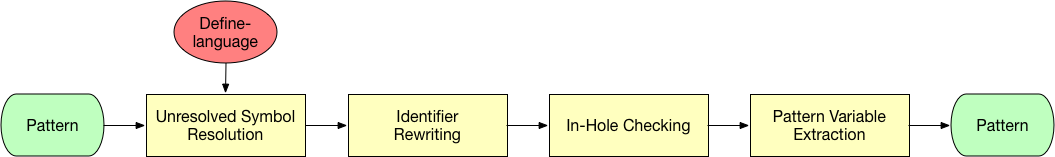
\includegraphics[scale=0.32]{pipeline-pattern-strat-2.png}

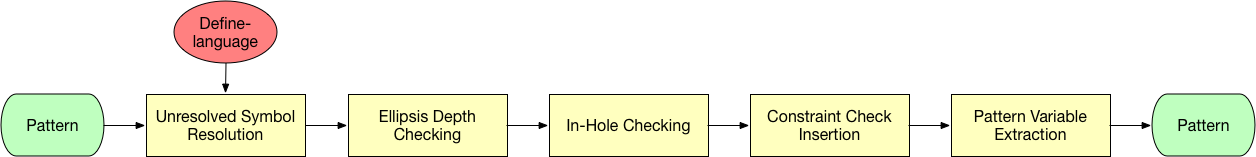
\includegraphics[scale=0.32]{pipeline-pattern-strat-3.png}

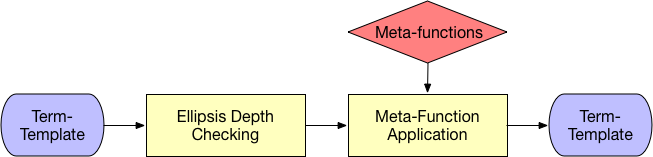
\includegraphics[scale=0.32]{pipeline-term-strat.png}

Notice that non-terminal resolution occurs with respect to non-terminal definitions on some \DefineLanguageNoArg form. Similarly, during "Metafunction Application Rewriting" pass requires set $Mf$ containing all meta-functions defined until this point. 

\begin{enumerate}
\item All $tl=$\TlDefineLanguage \space forms. Maintain a set $L$ that stores ($n, tl$) pairs.
\item All $tl=$\TlDefineMetafunction \space forms. Maintain a set $M$ that stores $(n, tl)$ pairs.
\item All $tl=$\TlDefineReductionRelation \space forms. Maintain a set $R$ that contains $(n, tl)$ pairs.
\end{enumerate}

\subsection{Top-Level Form Analysis}

\begin{itemize}
\item
Given $tl=$\TlDefineLanguage
	\begin{enumerate}
		\item apply strategy (1) to $tl$ resulting in $tl^{\prime}$.
		\item $L = L \cup \{ (n, tl^{\prime}) \}$
		\item Return $tl^{\prime}$.
	\end{enumerate}

\item $tl=$ \TlDefineMetafunction:
	\begin{enumerate}
	\item Ensure that there exists tuple $(l, tl) \in L$, otherwise raise Exception.
	\item apply strategy (2) to $domain$ and $codomain$ patterns resulting in $domain^\prime$ and $codomain^\prime$.
	\item For each $mc_i=$ \MetafunctionCase, apply strategy (3) to $p$ thus resulting in $p^{\prime}$ and apply term-processing strategy to $t$ resulting in $t^{\prime}$. Let $mc_i^{\prime}$ = \MetafunctionCase[$p^{\prime}$][$t^{\prime}$].
	\item Let $tl^\prime$  = \TlDefineMetafunction[$n$][$l$][$domain^\prime$][$codomain^\prime$][$mc_1^\prime$][$mc_n^\prime$][false].
	\item $M = M \cup \{ (n, tl^\prime)\}$ and return $tl^\prime$.
	\end{enumerate}

\item $red=$ \TlDefineReductionRelation:
\begin{enumerate}
\item ensure that there exists tuple $(l, df) \in L$ otherwise raise Exception.
\item Apply strategy (3) to $domain$ pattern resulting in $domain^\prime$, if it exists.
\item For each $rc_i=$ \ReductionCase \space in $r$, apply strategy (3) to $p$ resuling in $p^{\prime}$ and apply the only term-processing strategy to $t$ resulting in $t^\prime$. Let $rc_i^\prime=$\ReductionCase[$p^{\prime}$][$t^{\prime}$][$n$][false].
\item Let $tl^\prime=$\TlDefineReductionRelation[$n$][$l$][$domain^\prime$][$rc_1^\prime$][$rc_n^\prime$]
\item $R = R \cup \{ (n, tl^\prime) \}$ and return $tl^\prime$.

\end{enumerate}

\item $tl=$ \ReadFromStdinAndApplyReductionRelation
\begin{enumerate}
\item If $mf$ is present, ensure there exists tuple $(f, mf) \in M$, otherwise raise Exception.
\item Ensure there exists tuple $(r, red) \in R$, otherwise raise Exception.
\item Return $tl$.
\end{enumerate}


\item
$r=$ \RedexMatchAssertEqual.
	\begin{enumerate}
	\item Ensure that there exists tuple $(l, d) \in L$, otherwise raise Exception.
	\item Process $p$ according to strategy (3) resulting in $p^\prime$.
	\item Process $t$ according to the only specified strategy, resulting in $t^\prime$.
	\item For each $m_i=$ \Match, process each $t_i$ according to the only specified strategy resulting in $t_i^\prime$. Let $m_i^\prime=$\Match[$s_1$][$t_1^\prime$][$s_n$][$t_n^\prime$][false].
	\item Let $tl^\prime$=\RedexMatchAssertEqual[$l$][$p^\prime$][$t^\prime$][$m_1^\prime$][$m_n^\prime$][false] and return $tl^\prime$.
	\end{enumerate}

\item $tl=$ \TermLetAssertEqual
	\begin{enumerate}
	\item  Process each $t_i$ according to the only specified strategy resulting in $t_i^\prime$.
	\item Process $t$ and $e$ according to the only specified strategy, resulting in $t^\prime$ and $e^\prime$, respectively.
	\item Let $tl^\prime=$\TermLetAssertEqual[$v_1$][$n_1$][$t_1^\prime$][$v_m$][$n_m$][$t_m^\prime$][$t^\prime$][$e^\prime$][false] and return $tl^\prime$.
	\end{enumerate}

\item $tl=$ \ApplyReductionRelationAssertEqual
	\begin{enumerate}
	\item Ensure that there exists tuple $(r, red) \in R$, otherwise raise Exception.
	\item Process $t$ according to the only specified strategy resulting in $t^\prime$
	\item Process each term $e_i$ according to the only specified strategy, resulting in $e_i^\prime$.
	\item Let $tl^\prime=$\ApplyReductionRelationAssertEqual[$r$][$t^\prime$][$e_1^\prime$][$e_n^\prime$][false] and return $tl^\prime$.
	\end{enumerate}
\end{itemize}

\subsection{Remarks}
It should be noted that the way in which PyPltRedex handles metafunction resolution is slightly different from PLTRedex. PLTRedex seems to keep track of metafunctions that have been defined up until a certain point, and it also keeps track of metafunctions that have not been defined yet. Roughly speaking, instead of passing a single set $Mf$ into "Metafunction Application Pass", PLTRedex passes a second set $\overline{Mf}$ containing names of metafunctions that haven't been defined yet. This way, when attempting to detect metafunction applications, "Metafunction Application Pass" also checks set $\overline{Mf}$ and raises \lstinline{cannot use metafunction before its definition} error. Since PyPltRedex doesn't handle this at this time, all possible metafunction applications do not get rewritten and thus more often than not $codomain$ check fails.


